\documentclass[10pt,a4paper]{article}

\usepackage[utf8x]{inputenc}
\usepackage{ucs}
\usepackage{amsmath}
\usepackage{amsfonts}
\usepackage{amssymb}
\usepackage{fullpage}
\usepackage[slovene]{babel}
\usepackage{graphicx}
\usepackage{multirow}
\usepackage{tabularx}
\usepackage{ifpdf}
\usepackage{listings}
\usepackage{xcolor}
\usepackage{hyperref}

\definecolor{Butter}{rgb}{0.93,0.86,0.25}
\definecolor{Orange}{rgb}{0.96,0.47,0.00}
\definecolor{Chocolate}{rgb}{0.75,0.49,0.07}
\definecolor{Chameleon}{rgb}{0.45,0.82,0.09}
\definecolor{SkyBlue}{rgb}{0.20,0.39,0.64}
\definecolor{LightBlue}{rgb}{0.80,0.80,0.99}
\definecolor{DarkSkyBlue}{rgb}{0.10,0.19,0.34}
\definecolor{Plum}{rgb}{0.46,0.31,0.48}
\definecolor{Aluminium4}{rgb}{0.46,0.46,0.48}
\definecolor{ScarletRed}{rgb}{0.80,0.00,0.00}
\definecolor{DarkScarletRed}{rgb}{0.40,0.00,0.00}

\lstset{
	numbers=left,                   % where to put the line-numbers
	numberstyle={\small},      % the size of the fonts that are used for the line-numbers
	keywordstyle=[1]{\color{DarkSkyBlue}},
	keywordstyle=[2]{\color{DarkScarletRed}},
	keywordstyle=[3]{\bfseries},
	keywordstyle=[4]{\color{DarkPlum}},
	keywordstyle=[5]{\color{SkyBlue}},
	commentstyle={\color{Aluminium4}},
	stringstyle={\color{Chocolate}},
	basicstyle={\ttfamily\small},
	xleftmargin=17pt,
	breaklines=true,
	inputencoding=utf8x, 
	extendedchars=\true,
	frame=single
}



\pagestyle{empty}

\begin{document}

\begin{titlepage}
\begin{center}

% Upper part of the page

\includegraphics{Screenshot.png}\\[4.0cm]    
\textsc{\Large Dokumentacija}\\[4.5cm]

% Title
\hrule \ \\[0.2cm]
{ \huge \bfseries Navidezna fakulteta v WebGLu}\\[0.3cm]
\hrule \ \\[4.5cm]

% Author and supervisor
\begin{minipage}{0.4\textwidth}
\begin{flushleft} \large
\emph{Avtorji:}\\
Miha \textsc{Zidar}\\
Anže \textsc{Pečar}\\
Aleksandra \textsc{Bersan}\\
\end{flushleft}
\end{minipage}
\begin{minipage}{0.4\textwidth}
\begin{flushright} \large
\end{flushright}
\end{minipage}
\vfill

% Bottom of the page
{\large \today}
\end{center}
\end{titlepage}
\pagebreak
\section{Opis rešitve}
\subsection{Kaj rešitev sploh je}
Vsi vemo, da ima naša fakulteta zelo nelogično razporejene prostore in pogosto 
se zgodi, da obiskovalec ne najde prave predavalnice. Da bi obiskovalcem in 
brucom olajšali življenje, smo se odločili narediti 3-D model fakultete.\\\\
Ker želimo, da bi bila naša aplikacija čim lažje dostopna, smo jo postavili na 
internet s pomočjo odprtokodne knjižnice WebGL. Potrudili smo se, da aplikacija 
teče tekoče na sodobnih brskalnikih z WebGL podporo.
\subsection{Uporabljene metode}
\begin{center}

\includegraphics{./WebGL.png}
\end{center}
\subsection*{Jeziki}
\begin{itemize}
	\item \verb|JavaScript| - Delo z gl knjižnico
	\item \verb|GLSL| - za Fragment in Vertex shaderja
	\item \verb|Python| - Backend, pretvarjanje .obj datotek v json
\end{itemize}
\subsection*{Ogrodja}
\begin{itemize}
	\item \verb|webql-utils| - Za funkcijo requestAnimFrame
	\item \verb|glMatrix| - Uporabne funkcije nad matrikami in vektorji
	\item \verb|jQuery| - Izboljšanje uporabniške iskušnje
	\item \verb|Django| - Backend za shranjevanje podatkov o mestih zanimanja v podatkovno bazo 
\end{itemize}
\subsection*{Orodja}
\begin{itemize}
	\item Blender - Modeliranje faksa po gradbenih načrtih
	\item Gimp - Izdelava tekstur
\end{itemize}
%\subsection*{Metode}
\subsection*{Algoritmi}
\begin{itemize}
	\item Mipmap teksture
	\item Phongov odbojni model
	\item Collision detection
\end{itemize}
\pagebreak
\section{Zabavni deli}
\subsection{Collision detection}
V našem modelu imamo zaradi lažjega risanja v wegGL, vse ploskve predstavljene s trikotniki in ne s štirikotniki. To pa tudi nekoliko olajša detekcijo trkov med posameznimi površinami. Ponavadi se detekcijo trkov, hrani posebna podatkovna struktura, ki ima enako 3D predstavitev, vendar je načeloma razdeljena na manjše dele kot prvotna 3D mapa. Tukaj je tudi vprašanje, ali se nam splača hraniti dve strukturi ali samo eno. Mi smo se pri tej seminarski nalogi odločili da bomo imeli dve ločeni strukturi:
\begin{itemize}
\item faks: podatkovna struktura z velikimi poligoni in manj oglišči, ki se bo izrisovala 
\item coll: podatkovna struktura, ki je sestavljena iz veliko več manjših poligonov, ki se bojo uporabljali za detekcijo trkov.
\end{itemize}
Ponavadi so najbolj priljubljene strukture za zaznavanje trkov 
\begin{itemize}
\item KD-tree - k dimenzionalno drevo ki prostor na vsakem nivoju razdeli na dva dela glede na trenutno dimenzijo.
\item BSP-tree - struktura podobna kot KD-tree, vendar da na vsakem nivoju bolj optimalno razdeli prostor.
\item R-tree - drevo ki prostor razdeli na bounding box-e in se nato išče točke znotraj teh.
\item PR-tree - prioritetno R-tree, ki je le nadgranja R-tree da je iskanje hitrejše.
\end{itemize}
In tako kot so vse te strukture dobre za splošno iskanje trkov enega predmeta z ostalimi predmeti v prostoru, si lahko za naše potrebe izberemo kakšno, ki je malo bolj enostavna. To lahko rečemo, ker ne bomo veliko leteli (ko se leti, bo collision detection izklopljen), ali skakali. Torej to pomeni da bomo vedno v stiku z vsaj eno ploskvijo (tla), ter morda še z kakčno steno ali drugim objektom.\\
Torej ko smo se odločili za našo \verb|coll| strukturo, smo upoštevali kakšne so naše zahteve za detekcijo trkov in smo jo naredili tako da je največji trikotnik manjši ali enak objektu ki bo predstavljal čoveka, ki se sprehaja po faksu. V nadaljevnju bomo videli, da ni potrebno, da bi bili poligoni še manjši, čeprav so lahko nekateri, ki sestavljalo majhne natančne dele modela.
\subsubsection*{Struktura - navadena 2D tabela}
Na koncu smo videli da bo najlažje implementirati navadno 2D tabelo, ki bo imela naslednjo strukturo


\[
\begin{array}{l|l}
Index     & Value \\
0    & \lbrace x_0^0 \ldots x_m^0 \ | \ m\leq n  \rbrace \\
1    & \lbrace x_0^1 \ldots x_m^1 \ | \ m\leq n  \rbrace \\
2    & \lbrace x_0^2 \ldots x_m^2 \ | \ m\leq n  \rbrace \\
 \vdots   & \vdots \\
n    & \lbrace x_0^n \ldots x_m^n \ | \ m\leq n  \rbrace \\
\end{array}
\]
V kateri Index predstavlja zaporedno število posameznega trikotnika, in v Value je zapisan seznam indeksov ostalih trikotnikov, ki so zelo blizu trenutnega. Podatke o posameznem trikotniku lahko preberemo iz naše prejšnje strukture \"coll\" in indeksom trikotnika o katerem želimo podatke.\\

Sedaj pa potrebujemo le še manjšo strukturo, v kateri je seznam trikotnikov z katerimi se že dotikamo. To strukturo bomo pa imenovali "Touching". Celoten algoritem pa zgleda tako:
\begin{enumerate}
\item začetni položaj je na točno določenem trikotniku, in indeks tega trikotnika damo v Touching seznam.
\item shranimo trenutni položaj
\item premaknemo se na željeno mesto (kamor želi uporabnik).
\item za vsak indeks trikotnika ki je shranjen v Touching preverimo če se seka z našim osebkom.
\item preverimo tudi za vse indekse trikotnikov ki se nahajajo v seznamu trenutnega Touching trikotnika.
\item trikotnike katerih se dotikamo damo v Touching in tiste, ki se jih ne, damo ven. 
\item popravimo premik, če je potrebno in nadaljujemo pri točki 2.
\end{enumerate}

\subsubsection*{Algoritem - hitra detekcija trkov dveh trikotnikov}
Za detekcijo ne pregledujemo bounding boxov posameznih trikotnikov, in struktur, saj smo pri postavljanju strukture zagotovili da ne bomo pregledovali nobenih trikotnikov ki so nam predaleč.\\
Ugotavljanje pa poteka tako:
\begin{enumerate}
\item izračunaj enačbo ravnine za vsak trikotnik. 
\item naredimo skalarni produkt normale ravnine z vektorjemo od poljubne točke na ravnini do vsake točke na drugem trikotniku. Tako bojo imele točke na eni strani ravnine en predznak, točke na drugi strani pa drug predznak.
\item pogledamo če imajo vse točke enak predznak, kar pomeni da en trikotnik leži v celoti nad ali pod ravnino drugega trikotnika. V temu primeru ne more priti do trka in vrnemo 0.
\item enako naredimo tudi za drugi trikotnik.
\item pogledamo če so vse razdalje toče enega trikotnika od ravnine drugega trikotnika enake 0. in vrnemo da ni prišlo do trka. ker se tako znebimo dodatnih težav.
\item če oba trikotnika sekata ravnino drugega trikotnika, pa lahko naredimo črto presečišča ravnin in vemo da se laho trikotnika sekata le na tisti črti.
\item izračunamo presečišče stranic trikotnika z črto ki je je na presečišču ravnin, za oba trikotnika.
\item sedaj pa le pogledamo na tej premici če se intervala posameznih trikotnikov sekata, in v temu primeru vrnemo da je prišlo do trka
\end{enumerate}

Obravnavanje trkov pa je tudi enostavno, saj imamo shranjeno zadnjo dovoljeno pozicijo in nimamo nobenih prožnih odbojev. Edina posebnost je le da ko izvemo za vse ploskve s katerimi je prišlo do trka, bomo naš objekt premaknili v smeri seštevka normaliziranih normal teh ploskev. to nam bo omogočalo da hodimo v klanec in po stopnicah. 

\subsection{Pretvarjanje iz .obj v json in parsanje}
Za izrisovanja modelov iz Blenderja je potrebno prebrati datoteko v .obj formatu in iz zapisa
izluščiti $vertexe$, $normale$, $face$ in različne materiale. Za ta namen smo 
napisali preprosto python skripto, ki .obj datoteko prebere in prebrane podatke 
zapiše v json formatu. Na ta način smo pohitrili začetek izrisovanja, saj spletnemu
brskalniku ni potrebno parsati .obj datoteke ob vsaki naložitvi strani.
\pagebreak
\section{Problemi}
\subsection{Blacklisted GPUs}
Še preden smo začeli z razvojem naše seminarske naloge, smo naleteli na probleme.
Tako Googlov Chrome, kot Mozillin Firefox sta imela na črni listi grafične kartice,
ki so bile v naših računalnikih, kar je pomenilo, da je bil WebGL onemogočen. 
WebGLa ni bilo možno prisiliti k delovanju iz nastavitev znotraj brskalnika pa 
čeprav smo šarili po nastavitvah za developerje (Chromov: \verb|about:flags| in FFjev: \verb|about:config|).
Po nekaj dneh Googlanja smo le naleteli na sistemsko spremenljivko \verb|MOZ_GLX_IGNORE_BLACKLIST=1|,
s katero smo omogočili WebGL znotraj FireFoxa in Chromovo \verb|--ignore-gpu-blacklist| zagonsko stikalo.\\\\
Z najnovejšo različico Google Chromea nastavljanje zagonskega stikala ni več potrebno, 
FireFox4 pa še vedno potrebuje nastavljeno sistemsko spremenljivko.
\subsection{WebGL}
Začetnikom v OpenGLu iz lastnih izkušenj ne priporočamo dela z WebGLom. WebGL namreč temelji
na \verb|OpenGL ES 2.0|, ki je oskrunjena verzija OpenGLa, saj so iz specifikacije odstranili
vse funkcije iz OpenGLa, ki so v pomoč začetnikom. Brez dodatnih knjižnic WebGL ne
omogoča niti funkcij za skalarni ali vektorski produkt med vektorji, kaj šele funkcije
za translacije in rotacije matrik.
\subsection{Lepljenje tekstur}
Za lepljene tekstur smo sprva poskušali različne načine izvoza modelov iz Blenderja. Najbolj pogost izvoz ki se uporablja za WebGL je collada, ki pa nam brez posebnega ogrodja ne pusti veliko svobode pri programiranju - da bi pa naredili sami  svoj framework kot je naprimer spiderGL ali podobno pa nimamo časa. Torej smo se odločili da bomo zadevo izvažali v .obj format. Ta format lepo podpira tudi izvoz UVmap, ki bi jih lahko nato porabili za lepljenje tekstur na posamezne stranice.
Problem pa je ker imamo zelo velik model v blenderju in bi bilo rezanje in lepljenje tekstur ročno malo preveč mučno delo, tako smo se zato, in tudi da se malo več naučimo, odločili da bomo sami naredili svoj UVmap glede na materjal. Materjal pa je v blenderju zelo lahko določati posameznim stranicam, in po dogovoru smo tudi rekli da bo ime materjala pomenilo ime slike z .jpg končico ki se uporabi za teksturo.\\

Končno lepljenje teksture pa smo naredili tako, da smo vzeli trikotnik, in naredili projekcijo na osnovno ploskev ki mu je najbližja. To pomeni na ploskev, ki ima najbolj podobno normalo trikotniku. Probavali smo tudi da nebi prihajalo do popačenj in da bi trikotnik rajči rotirali do najbližje ploskve, vendar pri temu nebi vedno dobili lepih stikov med posameznimi ploskvami, tako smo videli da je navadna projekcija več kot dovolj za osnovni model.  

\subsection{Zaplet v ekipi}
Zaradi nepredvidljivih nesreč, se je upočasnilo delo enega člana ekipe, zaradi česa je celoten projekt potekal počasneje kot smo sprva predvidevali, saj so morali ostali člani za nekaj časa prevzeti drugo delo. Menim da to sicer ni preveč vplivalo na razvoj izdelka, se pa pozna v detajlih, ki bi jih lahko drugače dodali in bi občutno izboljšali uporabniško izkušnjo. Kot prototip pa smo z izdelkom še zmeraj zelo zadovoljni, in estetika ne odraža ravno vsega česar smo se pri izdelavi projekta naučili.
\pagebreak
\section{Nadaljne delo}
\subsection{Podrobnosti na modelu}
Zaradi časovne stiske in zapletov v ekipi nam je zmanjkalo časa za dodajanje podrobnosti, kot so 
table, lijaki, koši za smeti in ostali predmeti v predavalnicah in na faksu. Prav
tako nam ni uspelo dokončati vseh nadstropij fakultete. 
\subsection{Boljše teksture}
Če bi imeli več časa, bi lahko ustvarili svoje teksture iz fotografij, ki bi 
jih posneli na fakulteti. Lahko bi pa tudi nadgradili izrisovanje iz Mipmapinga
na kaj bolj modernega. 
\subsection{Druge ideje}
Ena izmed idej je bila tudi, da bi omogočili prikaz jakosti WiFi signala v posameznih delih 
fakultete. Zabavno pa bi bilo tudi, da bi se prikazoval položaj vseh obiskovalcev, ki so trenutno
znotraj navidezne fakultete.
\pagebreak
\section{Posnetki zaslonov}
\ \\
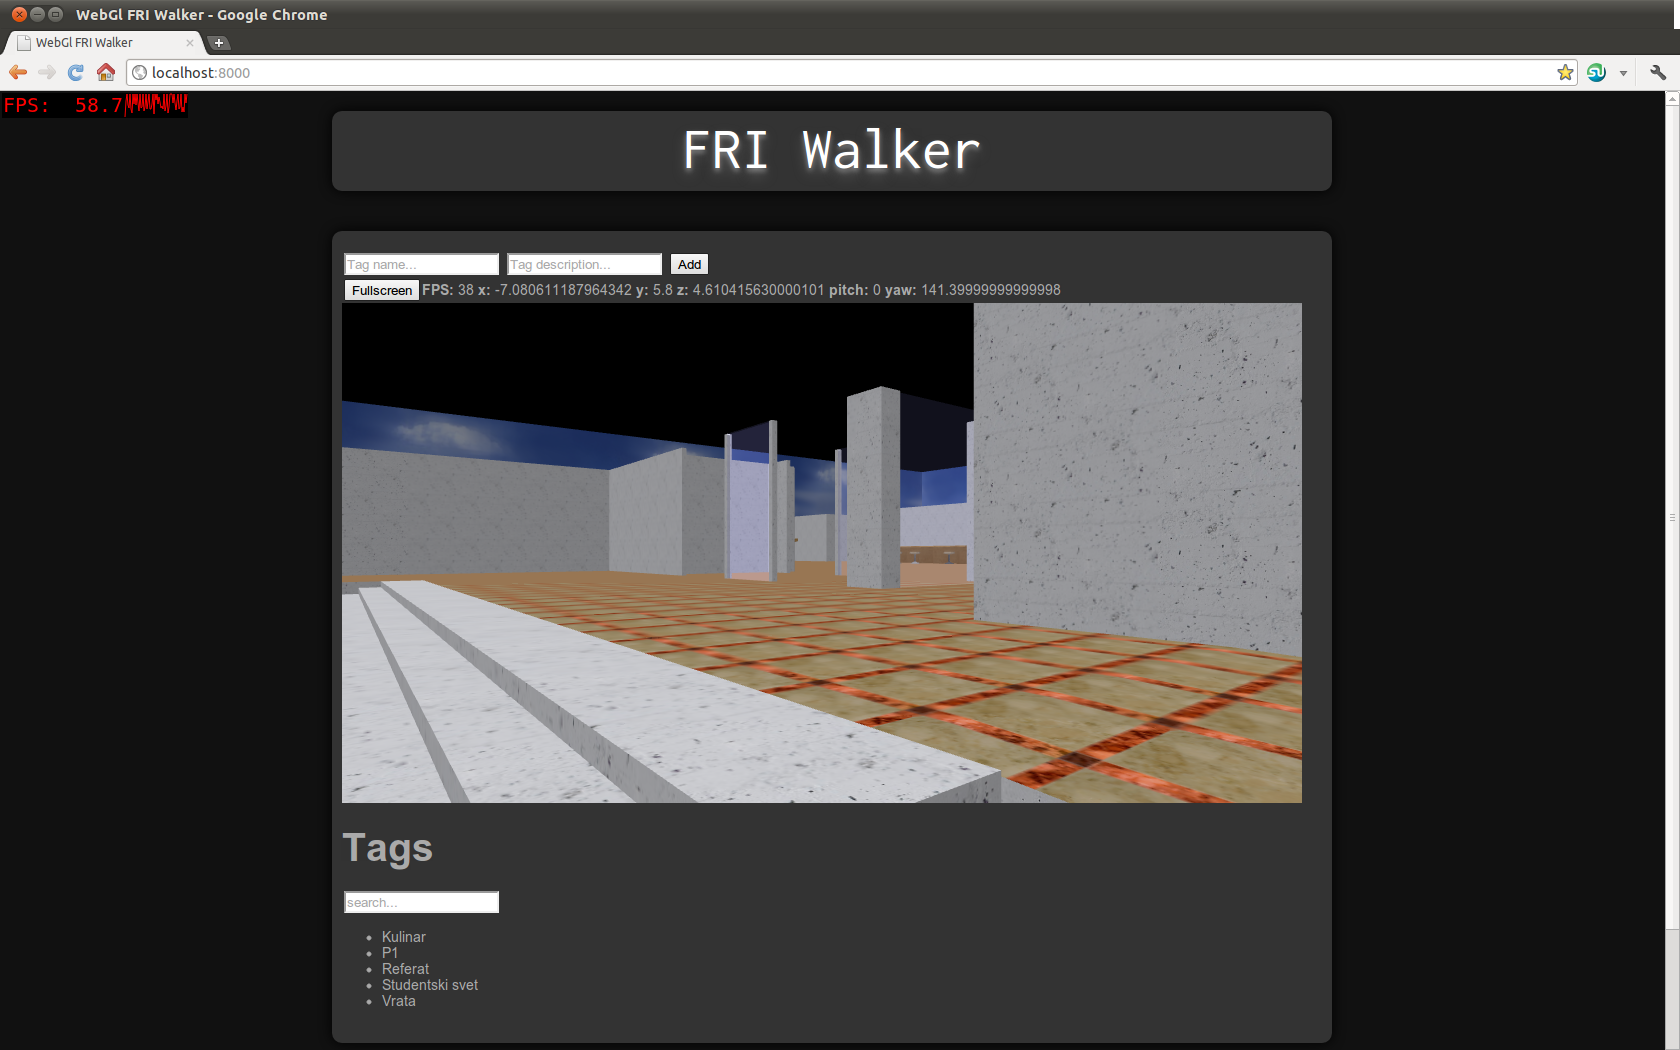
\includegraphics[scale=0.3]{screen1.png}\\ 

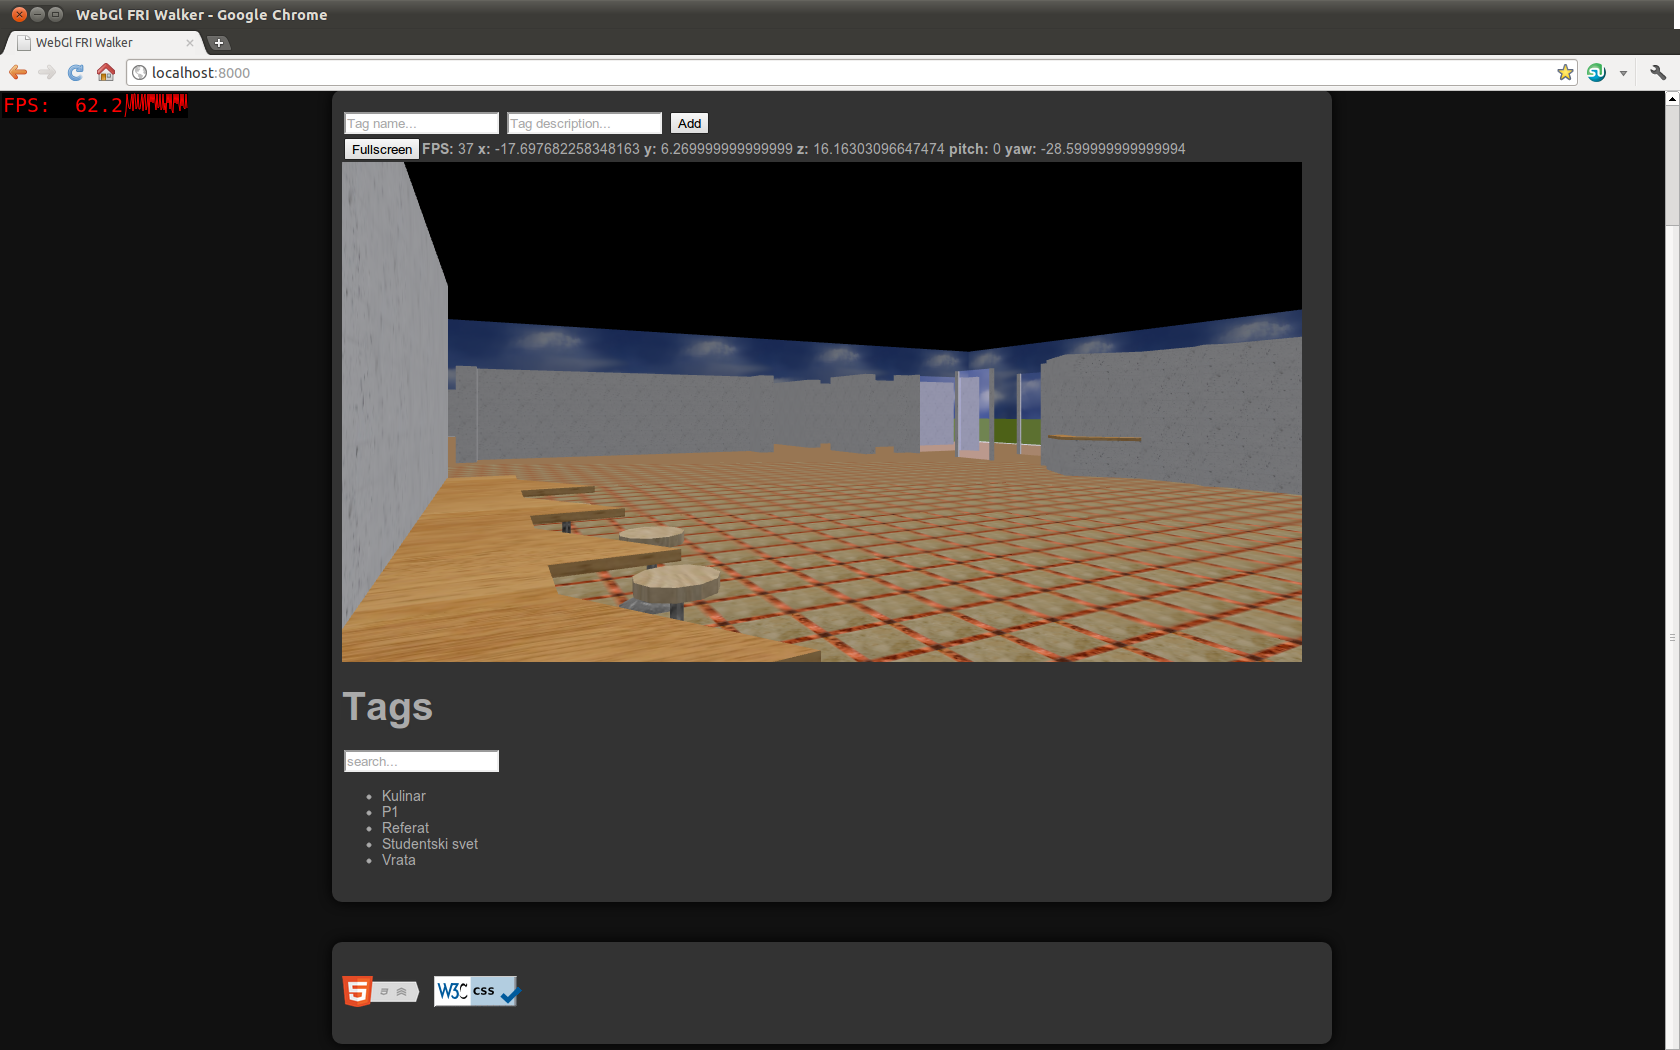
\includegraphics[scale=0.3]{screen2.png}\\

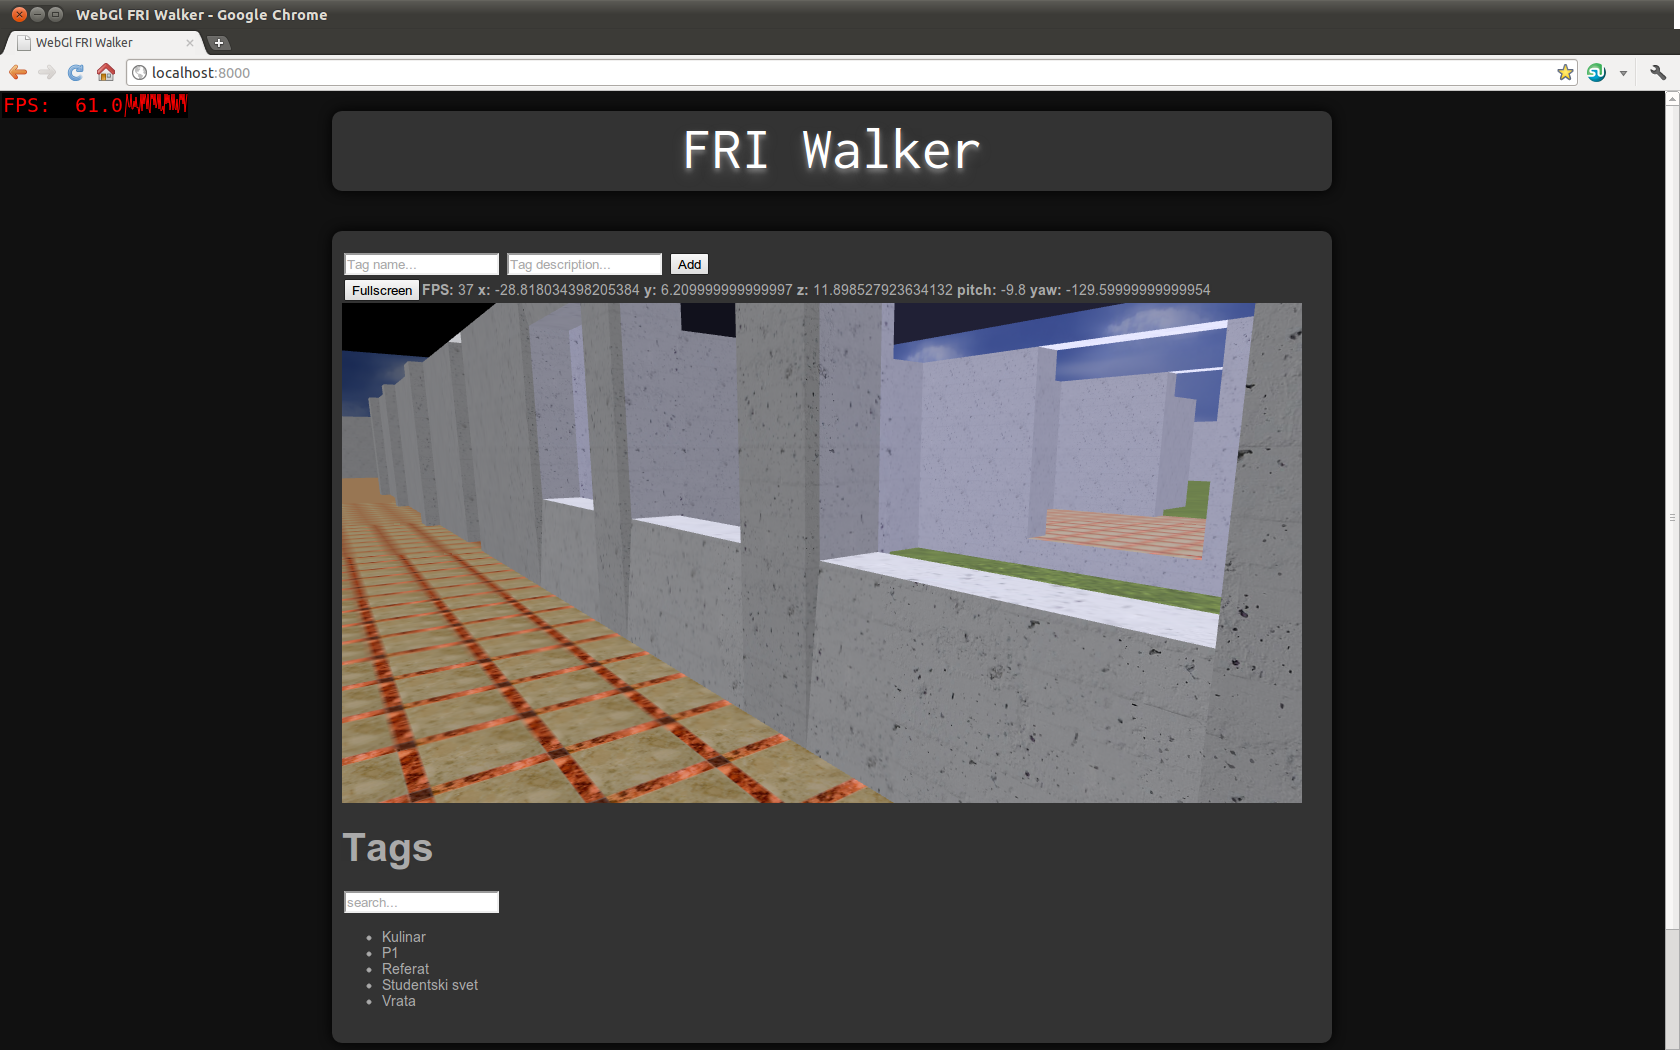
\includegraphics[scale=0.3]{screen3.png}\\

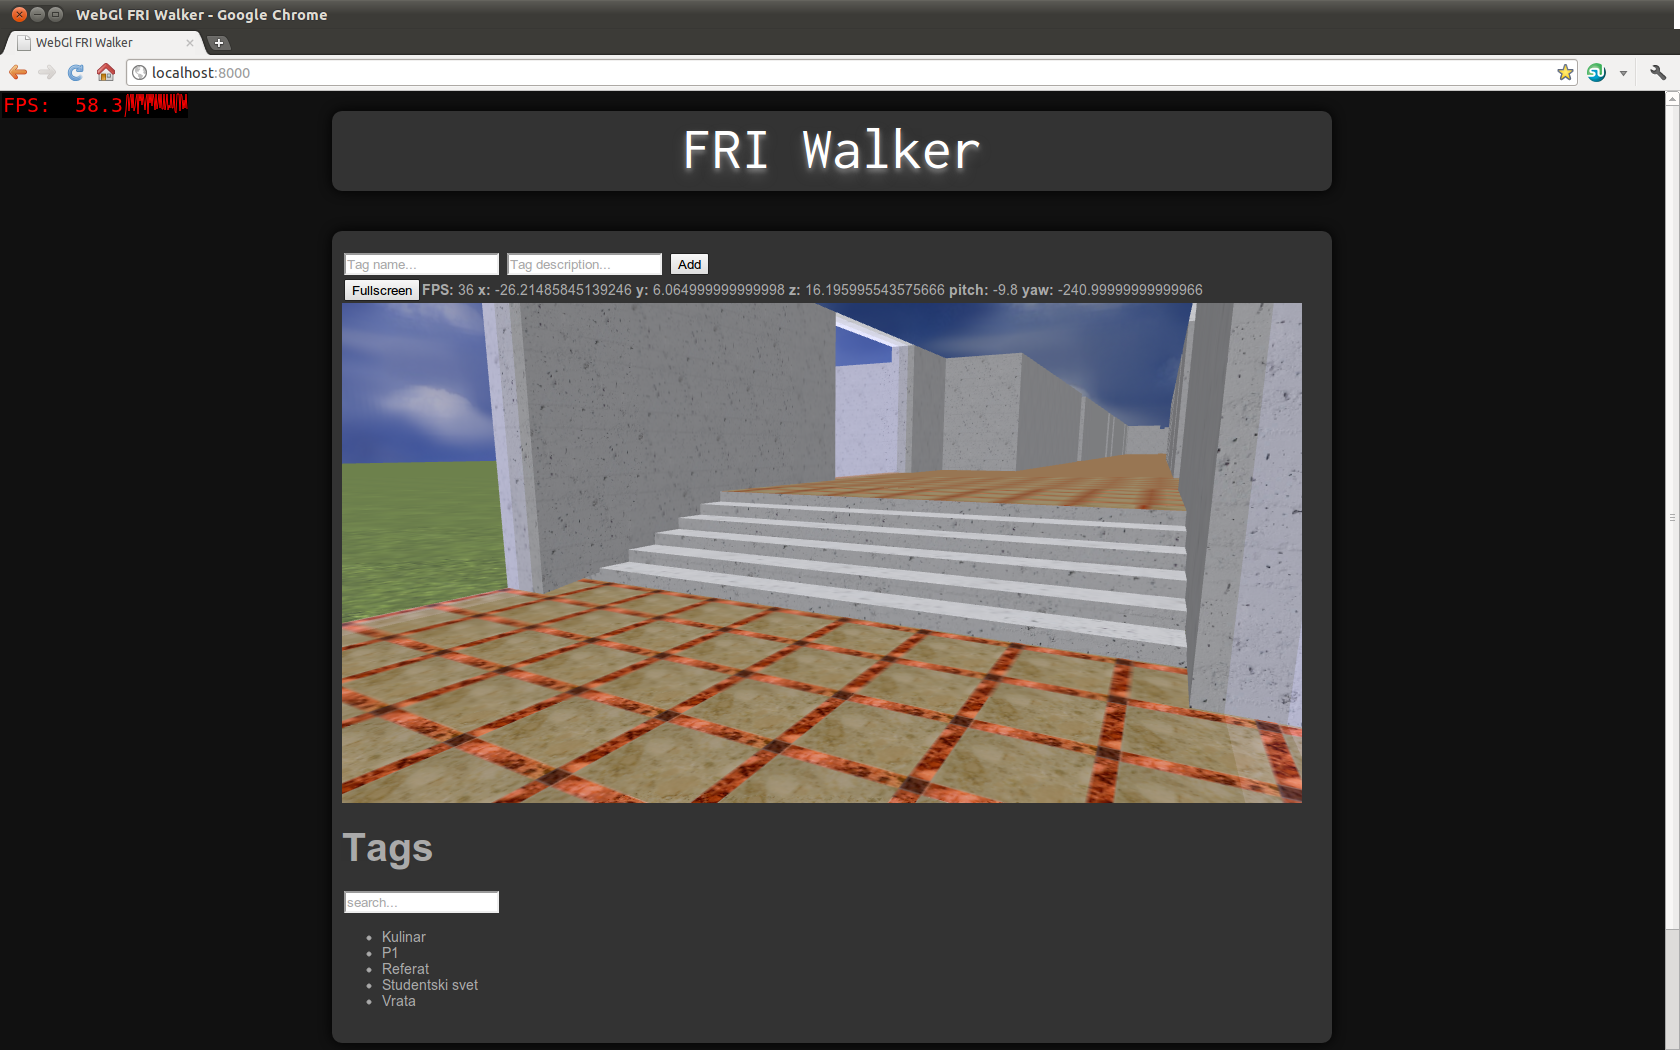
\includegraphics[scale=0.3]{screen4.png}\\
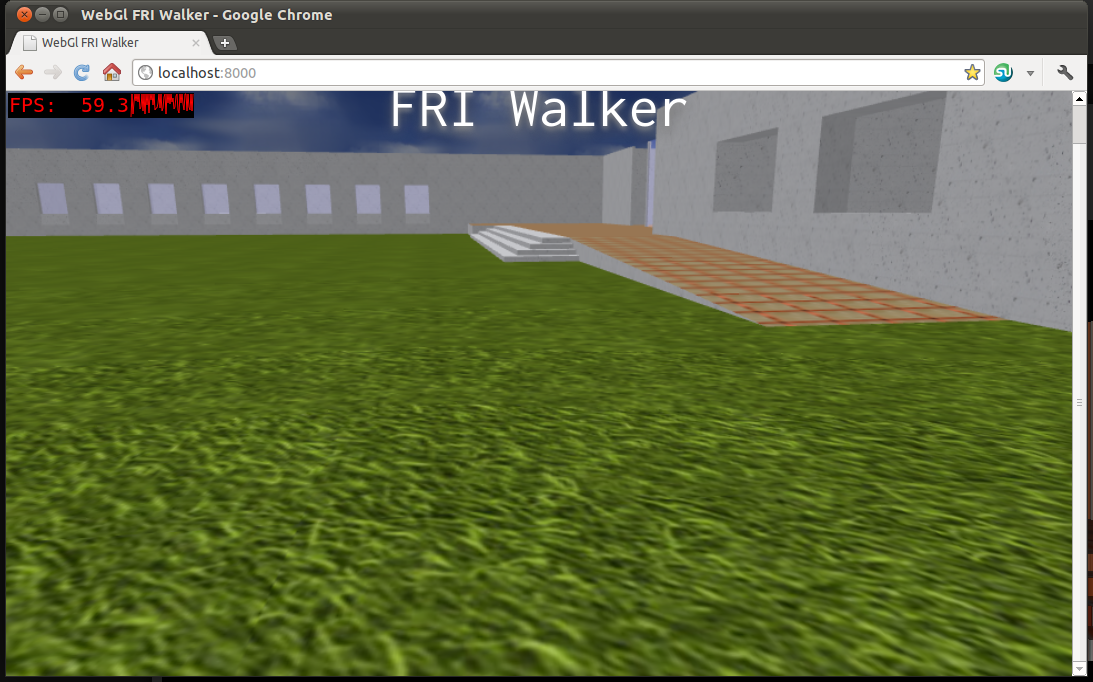
\includegraphics[scale=0.4]{screen5.png}\\ 

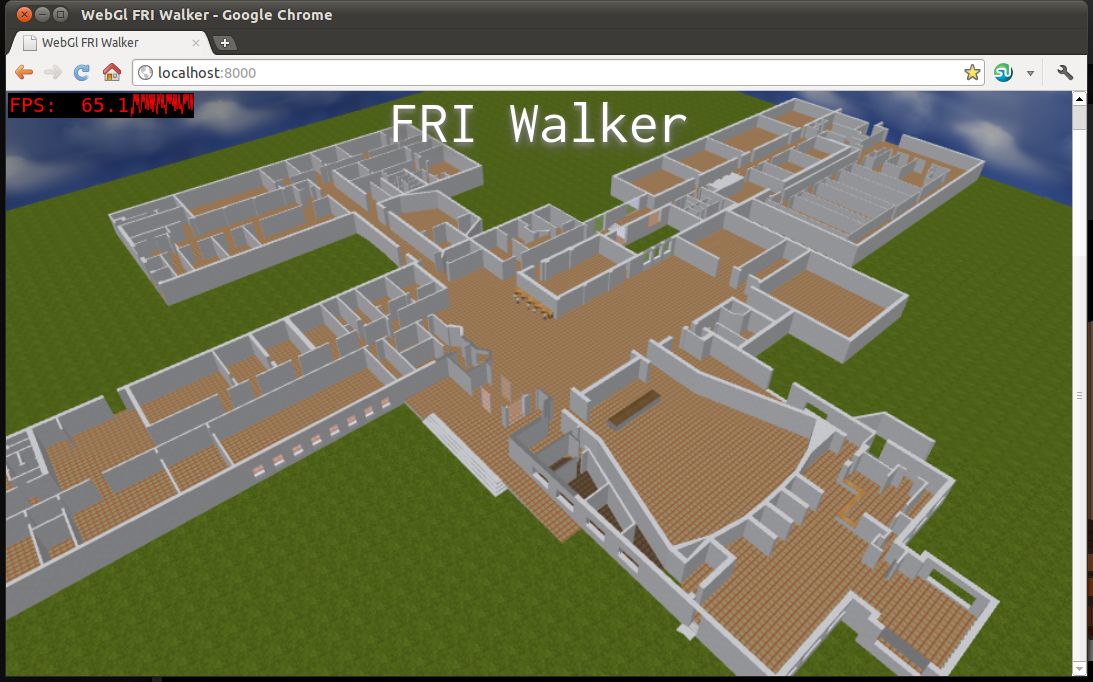
\includegraphics[scale=0.4]{screen6.png}\\ 

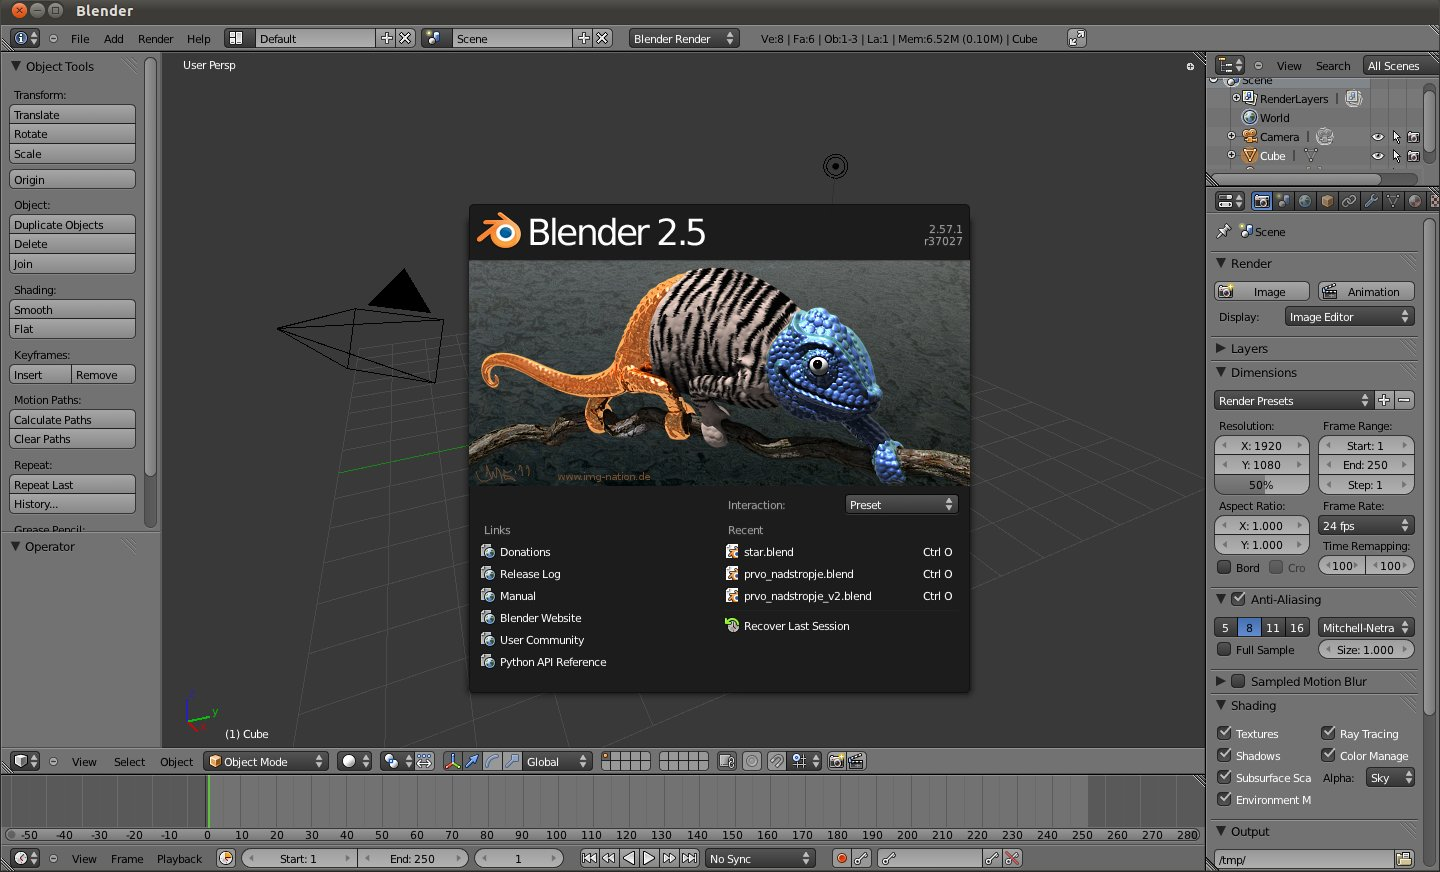
\includegraphics[scale=0.3]{Screenshot.jpg}\\ 
\ \\
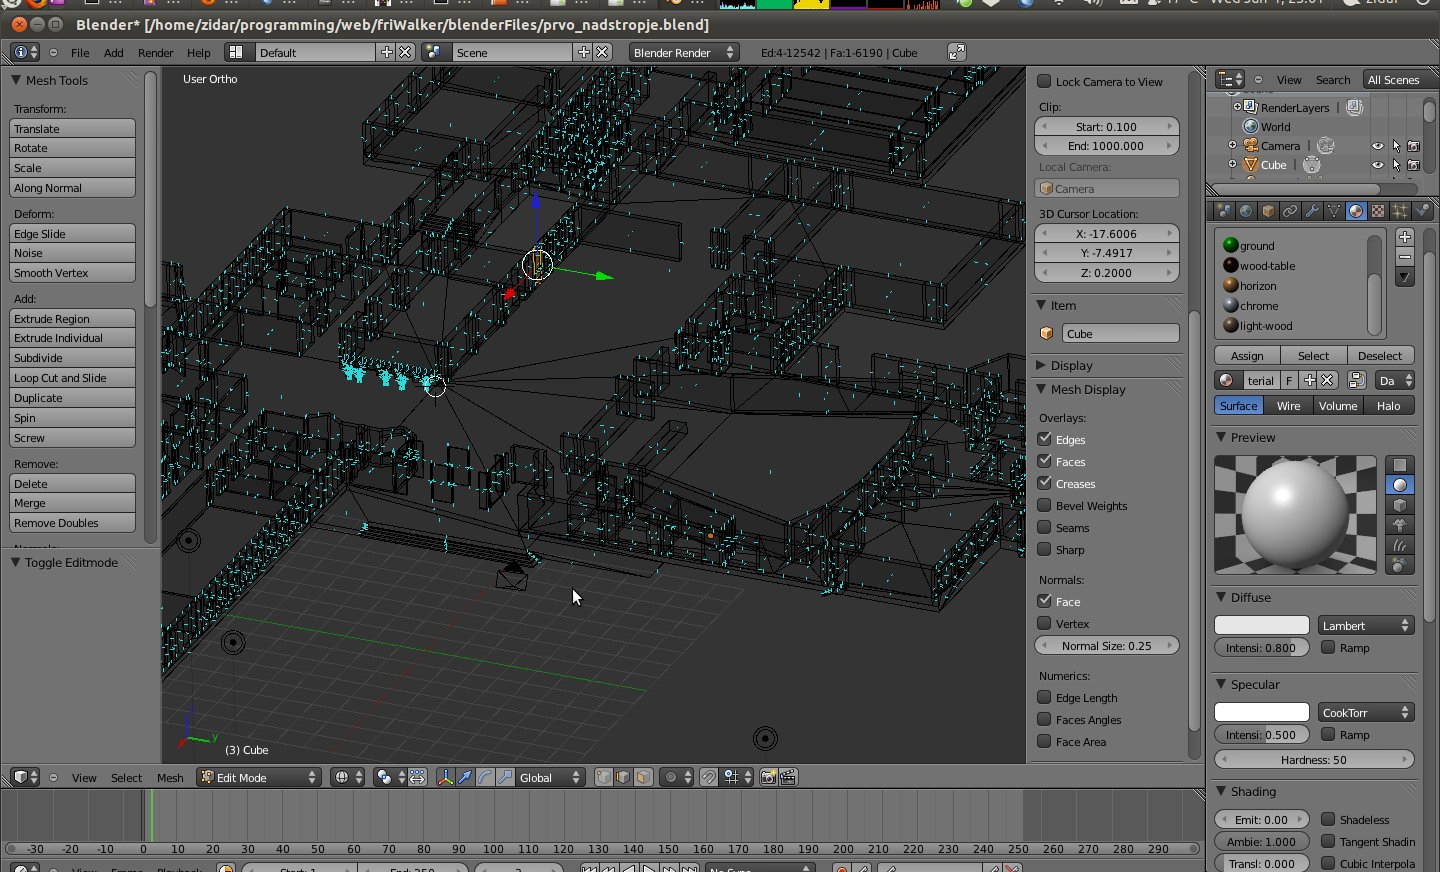
\includegraphics[scale=0.3]{Screenshot2.jpg}\\ 
\ \\
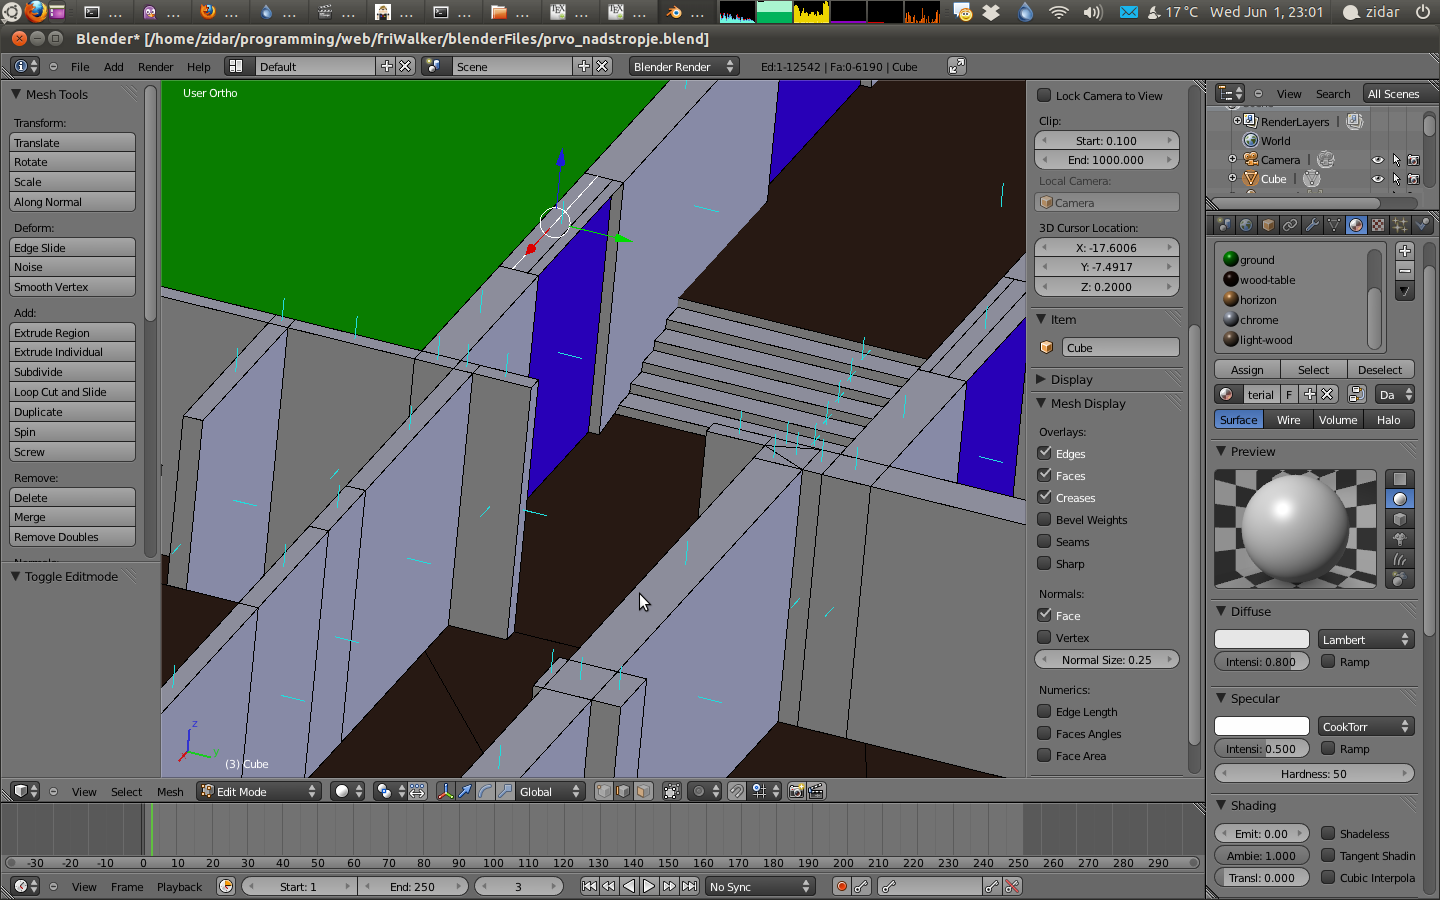
\includegraphics[scale=0.3]{Screenshot-1.png}\\ 
\ \\
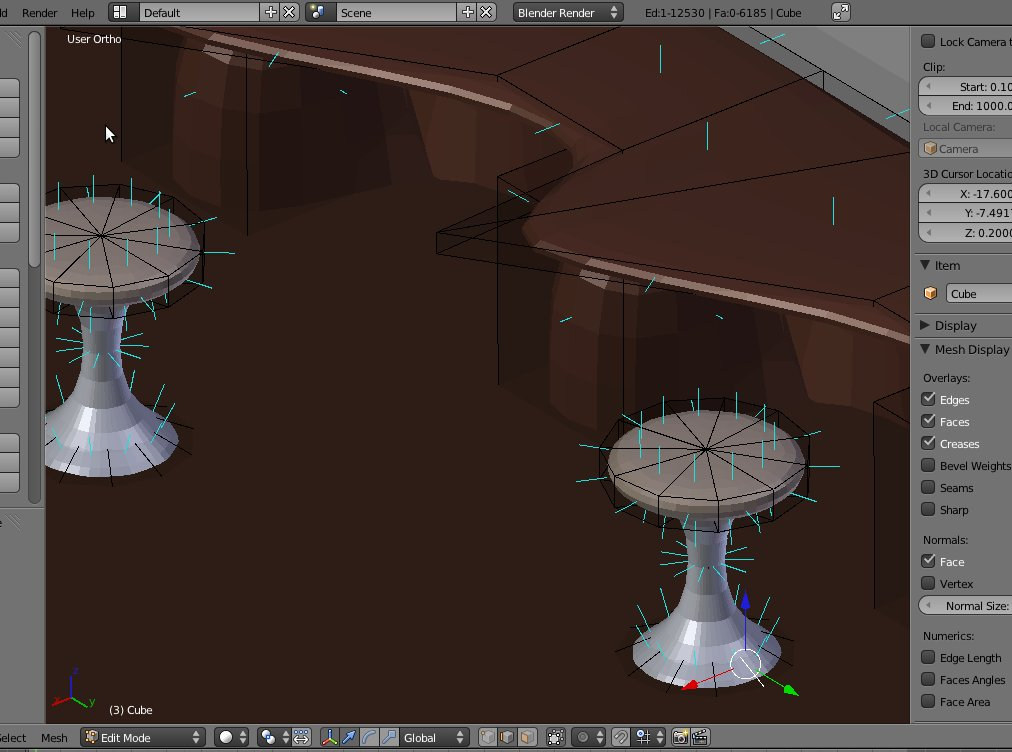
\includegraphics[scale=0.4]{Screenshot-3.jpg}\\ 
\ \\

\end{document}  %End of document.
